%% ICPRS 2027 -- 16th International Conference on Pattern Recognition Systems
%% IEEE conference format, 6 pages + 1 page of references. Build: tectonic -X compile icprs2027.tex
\documentclass[conference]{IEEEtran}
\IEEEoverridecommandlockouts

\usepackage{cite}
\usepackage{amsmath,amssymb}
\usepackage{graphicx}
\usepackage{textcomp}
\usepackage{booktabs}
\usepackage{url}
\usepackage[hidelinks]{hyperref}

\newcommand\blfootnote[1]{%
  \begingroup\renewcommand\thefootnote{}\footnote{#1}\addtocounter{footnote}{-1}\endgroup}
\begin{document}

\title{Annotation Convention, Not Architecture, Limits\\Cross-Facility Detection of Electric Vehicle\\Battery Components}

\author{
\IEEEauthorblockN{Komiljon Kosimov and Shiv Ashutosh Katiyar}
\IEEEauthorblockA{\textit{Department of Mechanical Engineering,
University of Birmingham}, Birmingham B15 2TT, United Kingdom \\
kxk445@student.bham.ac.uk, ~ s.a.katiyar@bham.ac.uk}
}

\maketitle
\blfootnote{Benchmark definition, per-source provenance and licence record, audit tooling, evaluation code and detector weights: \url{https://github.com/Komil-jon/ev-battery-vision-pipeline}}

\begin{abstract}
Automated disassembly of end-of-life electric vehicle (EV) battery packs depends on a
detector that locates modules and busbars across the pack types a recycling line
actually receives. Published detectors for this task are trained and validated at a
single facility. This paper assembles a cross-facility corpus from 13 independent
public sources spanning ten pack families, verified free of train-test leakage by
perceptual hashing, and disaggregates accuracy by source. Error proves concentrated
rather than spread: per-source module accuracy spans 0.097 to 1.000, and the collapse
occurs where a source disagrees about what the target class denotes rather than where
the imagery is difficult. This is developed into a screening procedure that identifies
convention-divergent sources from a single training run using a robust outlier
criterion, and into a training-free variant computed from annotation geometry alone
over 4,760 label files. Both pass a positive control in which a consensus source
relabelled to a sub-component convention is recovered while no other source changes
status. Two further results concern method rather than data. Under a matched 60-epoch
budget, self-supervised pretraining is marginally worse on conventionally annotated
packs, at 0.955 against 0.979, and better by a factor of 3.5 under annotation shift,
at 0.337 against 0.097. And validation data drawn from a single divergent source is
shown to \emph{invert} checkpoint selection rather than merely bias it: the selected
checkpoint is worse than the fixed-budget final checkpoint by 51\% relative, with
non-overlapping bootstrap intervals, in both architectures tested. Five negative
results are reported. The corpus definition and evaluation code are released.
\end{abstract}

\begin{IEEEkeywords}
object detection, dataset quality, annotation consistency, domain generalisation,
cross-dataset evaluation, electric vehicle batteries, circular economy
\end{IEEEkeywords}

\section{Introduction}

Electric vehicles are reaching end of life in large numbers, and the packs they
carry are simultaneously a hazard and a source of critical raw materials. Lithium,
cobalt and nickel are all classified by the European Commission as critical raw
materials with elevated supply risk \cite{ec_crm,harper2019}, and European
recycling capacity demand is projected to reach 170\,GWh by 2035 \cite{te2024}.
Disassembly of these packs remains predominantly manual. The operation is
labour intensive, slow, and exposes workers to high voltage and to the risk of
thermal runaway, which motivates a substantial and growing research effort on
robotic disassembly \cite{zang2024robotic,tan2025screws}.

Every such system begins with perception. Before a manipulator can unfasten,
grasp or lift a component, the battery modules and the busbars that connect them
must be located in the image. The established approach is a supervised object
detector trained on imagery collected at one facility or from one experimental
rig. This practice conceals a problem specific to the application. A recycling
line does not receive a single pack type; it receives whatever arrives on a given
day, from different manufacturers, in different states of disassembly, under
whatever illumination the building provides. Accuracy measured on the
distribution a detector was trained on therefore carries limited information
about the next pack through the door.

To quantify this, a cross-facility benchmark for EV battery component detection
is required, and none exists. Every study surveyed in
Section~\ref{sec:related} collected and annotated its own imagery, and none
released it. To address this gap, this paper assembles a corpus of 4,425
training images from 13 independent public sources spanning ten EV pack families,
constructs a held-out cross-facility benchmark of 225 images and 780 instances,
and evaluates detectors on it under a single harmonised protocol.

The principal finding is that the dominant failure mode is not image difficulty
and not model capacity. It is disagreement between sources about what the target
class denotes. Per-source module accuracy spans 0.995 to 0.043, and inspection
confirms that the collapsing source annotates small internal sub-components as
modules while every other source annotates pack-level modules. The detector
learned the majority convention and applied it consistently; the collapse is a
disagreement about the target, not a failure of perception.

This paper makes the following contributions:

\begin{enumerate}
\item A cross-facility corpus and benchmark for EV battery component detection,
assembled from 13 public sources over ten pack families, leakage-checked and released
with per-source provenance and licences (Section~\ref{sec:data}).
\item A convention-consistency screening procedure identifying annotation-divergent
sources from a single training run, with a positive control in which a relabelled
consensus source is recovered and no other source changes status
(Sections~\ref{sec:screen}, \ref{sec:res-screen} and \ref{sec:res-control}).
\item A training-free variant computed from annotation geometry alone, which
identifies the same source with no training run (Sections~\ref{sec:screen-free} and
\ref{sec:res-screen-free}).
\item A matched-budget architecture comparison showing self-supervised pretraining to
be marginally worse on conventionally annotated packs and better by a factor of 3.5
under annotation shift (Section~\ref{sec:res-arch}).
\item The finding that single-source validation \emph{inverts} checkpoint selection,
costing 51\% relative accuracy, in both architectures tested
(Section~\ref{sec:res-inversion}).
\item Five negative results constraining the design space
(Section~\ref{sec:negative}).
\end{enumerate}

\textbf{Relation to prior work by the same authors.} The single-source specialist
evaluated here is the detector of \cite{katiyar2026mvml}, which addressed detection
and condition assessment at one facility. That work could not test cross-facility
transfer, which is the limitation this paper addresses. The corpus, the benchmark,
both screening procedures and all evaluation reported here are new.

\section{Related Work}
\label{sec:related}

\subsection{Perception for battery disassembly}
Zang \emph{et al.} \cite{zang2024robotic} surveyed robotic EV battery disassembly
and concluded that the process remains predominantly manual, with perception and
task uncertainty identified as the principal obstacles. Wegener \emph{et al.}
\cite{wegener2015} demonstrated that pack designs vary sufficiently between
manufacturers that fixed automation does not transfer, which is the practical
reason perception must generalise. However, that study addressed mechanical
disassembly sequencing and did not evaluate a perception component.

Most published perception work for this application targets fasteners rather
than components. Screw detection has been addressed with Faster R-CNN combined
with rotation edge similarity \cite{screwrcnn2021}, with YOLOX-family detectors
\cite{screwbatt2023}, and in a recent comparison of YOLOv11 against Faster R-CNN
\cite{screwcompare2026}. However, each of these studies reports accuracy on
imagery from a single collection and therefore cannot establish transfer.
Module-level and busbar-level perception is comparatively under-explored. Tan
\emph{et al.} \cite{tan2025screws} developed a collaborative robot that unfastens
and collects screws by fusing vision with force and torque sensing, reporting
above 90\% unfastening efficiency; however, the vision component operates on a
single fixed pack geometry. The closest prior work applies instance segmentation
with point-cloud registration to grasp busbars \cite{cvmodule2023}, but is
restricted to one module type.

A recurring theme is data scarcity. Every study named above collected and
hand-annotated its own imagery, 1,719 images in the case of
\cite{screwbatt2023}, and none released it. \cite{screwcompare2026} resorts to
laptop screws as a proxy domain and states that the field is hampered by a lack
of public datasets. That absence motivates the benchmark presented here.

\subsection{Cross-dataset evaluation and label quality}
Domain shift is a well-documented failure mode in visual recognition
\cite{recht2019,koh2021wilds}: models that appear strong on their own test split
degrade sharply on data collected under a different protocol. However, these
benchmarks vary the imaging distribution while holding the annotation protocol
fixed, whereas the corpus considered here varies both. Northcutt \emph{et al.}
\cite{northcutt2021} demonstrated that pervasive label errors in established test
sets destabilise benchmark rankings, but treated label error as noise about an
agreed target rather than as systematic disagreement about what the target is.
The distinction matters for merged corpora, and it is the distinction the
proposed screening procedure operationalises. Penquitt \emph{et al.}
\cite{penquitt2026} developed a modular framework combining automatic label-error
detection with crowd-sourced verification, recovering 18\% missing or inaccurate
labels in the KITTI pedestrian class. However, that framework corrects errors
relative to a standard agreed within a single dataset, whereas the sources
considered here disagree about what the class denotes, which no within-convention
correction can reconcile. Abou Akar \emph{et al.} \cite{abouakar2026} studied
multi-source training for industrial detection using real, rendered and
generatively synthesised imagery. However, those sources share one annotation
standard by construction, since synthetic data carries its ground truth.

\subsection{Self-supervised representations for detection}
Benchmark design for industrial vision has precedent: MVTec AD
\cite{bergmann2019mvtec} established that a carefully constructed benchmark can
redirect a sub-field, though it was collected by one group under controlled
conditions and so exhibits no inter-source annotation disagreement. Zhou
\emph{et al.} \cite{zhou2022dg} surveyed domain generalisation; however, that
taxonomy presumes a fixed label space across domains, the assumption shown here to
fail on assembled corpora. Self-supervised backbones such as DINOv2 \cite{dinov2}
learn features that transfer without task-specific fine-tuning, and detection
transformers \cite{carion2020detr} built on them \cite{rfdetr} are reported to generalise better than detectors trained from
scratch in low-data regimes. However, that claim has been established on natural
imagery with consistent annotation. Whether it holds on the cluttered, specular
imagery of battery internals, and under annotation shift, is evaluated in
Section~\ref{sec:res-arch}.

To the best of our knowledge, no public cross-facility benchmark for EV battery
component detection exists, and no prior study has quantified the contribution of
annotation-convention divergence to cross-source detection accuracy. Therefore,
this research presents both.

\section{Corpus and Benchmark}
\label{sec:data}

\subsection{Sources}
A corpus of 4,425 training images was assembled from 13 independent public
sources spanning ten EV pack families, annotated with two classes,
\texttt{module} and \texttt{busbar} (Table~\ref{tab:sources}). The images and the
polygon annotations originate with those sources; the contribution made here is
the assembly, the deduplication, the audit and the benchmark construction, not
the annotation. Licences differ across sources and one is non-commercial, so
per-source provenance is recorded and released so that any single source can be
excluded by a downstream user.

\begin{table}[t]
\caption{Corpus sources (13 total, ten pack families)}
\label{tab:sources}
\centering\footnotesize
\setlength{\tabcolsep}{4pt}
\begin{tabular}{lrl}
\toprule
Source & Images & Pack family \\
\midrule
ev-battery-comp-det. & 1,045 & multi-manufacturer \\
ev-battery-components & 680 & Audi / BMW / Chevrolet \\
last\_exp4 & 483 & multi-manufacturer \\
ev-battery-pack & 435 & single laboratory rig \\
battery\_comp, ue\_d1 & 517 & Nissan Leaf, close-ups \\
Others (eight sources) & 1,265 & mixed \\
\bottomrule
\end{tabular}
\end{table}

\subsection{Deduplication and leakage control}
Reported accuracy is informative only against a benchmark that does not overlap
the training data. All 4,440 candidate images were therefore compared by
difference hashing (dHash) at a Hamming distance threshold of 6, a value selected
because it separates augmentation-derived near-duplicates from genuinely distinct
frames on this corpus. Fifteen same-source near-duplicates were removed, and a
cross-source pass at a looser threshold returned zero duplicates, which confirms
that the sources are genuinely independent rather than republications of one
another.

This control proved necessary rather than precautionary. One candidate source, a
712-image public collection covering 19 vehicle types, republishes imagery from
another source already present in the corpus: 78 images were byte-identical
duplicates of training images. Merging without verification would have placed
training images directly into the benchmark.

\subsection{Annotation audit}
\label{sec:audit}
All 4,425 training images were audited for label and image quality. Of these,
23.5\% carry no labels, 12.3\% score low on a Laplacian-variance blur metric,
20.4\% are greyscale, and none contain degenerate boxes.

Two findings changed how the corpus was treated. Firstly, the blur and greyscale
flags are largely false alarms. The lowest-scoring images are smooth, closed pack
lids, for which a Laplacian-variance metric reads flat metal as blurred, and the
greyscale images originate from two monochrome sources. Both add useful
variation, so deletion on the metric alone would degrade the corpus. Secondly,
the harmful category is unlabelled images that nonetheless contain visible
components. A proportion of the 23.5\% is legitimate background, which suppresses
false positives, but inspection confirmed open packs with clearly visible busbar
assemblies carrying no annotations. Such frames teach the detector that busbars
are background and are a plausible contributor to the weak busbar accuracy
reported in Section~\ref{sec:res-arch}.

The audit also established that 16,945 of the 19,522 annotations are polygon
masks with between 5 and 151 vertices rather than boxes. These are converted to
enclosing boxes for detection training and evaluation. It should be noted that an
early version of the evaluation pipeline silently discarded every polygon-format
label, trained on 20\% of the annotations, and produced an inflated score that
appeared plausible. The failure is easy to introduce and difficult to detect, and
ground-truth instance counts should be reconciled across pipelines as a matter of
routine.

\subsection{The cross-facility benchmark}
A cross-facility benchmark of 225 images containing 780 instances was drawn from
all sources and held out entirely from training. A convention-consistent subset
of 177 images, obtained by applying the screening procedure of
Section~\ref{sec:screen}, is reported alongside it throughout.

\section{Method}

\subsection{Detectors and training configurations}
Three configurations are compared.

\textbf{Single-source specialist.} YOLOv8n trained only on the single-laboratory
source at 768\,px, following the conventional approach in this literature.

\textbf{Multi-source YOLO11n.} YOLO11n \cite{yolo11}, 2.6\,M parameters, trained
from COCO initialisation \cite{lin2014coco} on all 13 sources at 640\,px with SGD.

\textbf{Multi-source RF-DETR.} RF-DETR-Nano \cite{rfdetr}, a real-time detection
transformer \cite{carion2020detr} initialised from the published checkpoint, whose
backbone derives from self-supervised DINOv2 pretraining \cite{dinov2}, fine-tuned end
to end at 672\,px. All 30.6\,M parameters are updated; the backbone is not frozen.

\textbf{Matched budget.} An architecture comparison is meaningful only under
equivalent training. Both multi-source models are therefore trained for exactly 60
epochs at the closest resolutions the architectures accept, RF-DETR requiring a
multiple of 56. Early stopping is disabled and the final checkpoint taken, for the
reason established in Section~\ref{sec:res-inversion}. YOLO11n was trained with three
seeds; RF-DETR once at the full budget, a limitation stated in
Section~\ref{sec:limits}.

\subsection{Harmonised evaluation protocol}
Confidence scores are not comparable across architectures, and mixing metric
implementations produced a spurious result in early experiments conducted for
this study. Every model is therefore scored with a single metric implementation
at a common confidence threshold of 0.05, on identical images, against identical
ground truth including polygon-derived boxes. The threshold of 0.05 was selected
because it lies below the operating point of all three detectors and therefore
does not truncate the precision-recall curve for any of them.

\subsection{Convention-consistency screening}
\label{sec:screen}
The proposed screening procedure identifies sources whose annotation convention
diverges from the corpus consensus, using a single merged-corpus training run.

Let $\mathcal{S}=\{S_1,\dots,S_n\}$ denote the sources and let $a_i$ denote the
class-specific mAP@50 obtained by the merged-corpus detector on the held-out
images of $S_i$. A source is flagged as convention-divergent when its accuracy
falls below a robust lower fence,
\begin{equation}
a_i < \operatorname{med}(\mathbf{a}) - k \cdot 1.4826 \cdot \operatorname{mad}(\mathbf{a}),
\label{eq:screen}
\end{equation}
where $\mathbf{a}=(a_1,\dots,a_n)$, $\operatorname{med}$ denotes the median,
$\operatorname{mad}$ denotes the median absolute deviation, the constant 1.4826
rescales the median absolute deviation to a consistent estimator of the standard
deviation under normality, and $k$ is a sensitivity parameter. A value of $k=3$
is used throughout, which is the conventional choice for outlier rejection and
which is shown in Section~\ref{sec:res-screen} to separate the divergent source
from the consensus by a wide margin on this corpus.

The median and the median absolute deviation are used in place of the mean and
the standard deviation because a divergent source inflates both of the latter and
thereby masks itself. The procedure requires no additional annotation, no
additional training run beyond the merged-corpus model that is trained in any
case, and no assumption about which source is divergent.

Two conditions apply. A source must contribute at least 100 module instances to be
screened, below which it is excluded rather than reported; at 40 instances an earlier
evaluation produced a 0.36 mAP@50 swing on the smallest source between models
differing only in an unrelated source's labels. And the screen is computed on a
stratified sample of the corpus rather than held-out data, because it is a curation
diagnostic: a source contradicting the majority convention is not fitted well even in
training. Absolute values are consequently optimistic and only orderings are used.

A flagged source is not discarded from the corpus. It is reported separately as
an out-of-convention benchmark, on the grounds established in
Section~\ref{sec:res-screen} that its labels encode a different task rather than
a degraded version of the same one.

\subsection{Training-free screening from annotation geometry}
\label{sec:screen-free}
The procedure above requires a merged-corpus training run. A cheaper variant
operates on the annotation files alone. A source annotating sub-components rather
than pack-level modules produces many small boxes per image, whereas a source
following the consensus convention produces few large ones. That signature is
captured by a granularity index, defined as follows:
\begin{equation}
g_i = n_i / s_i ,
\label{eq:granularity}
\end{equation}
where $n_i$ denotes the mean number of module instances per image in source $S_i$
and $s_i$ denotes the median normalised module scale, taken as the square root of
the enclosing-box area in normalised image coordinates. Scale enters as a square
root so that the index is a count per unit length and is invariant to image
resolution. Eq.~\ref{eq:screen} is applied to $\mathbf{g}$ with the inequality
reversed, since divergence raises the index.

\section{Results}

\subsection{The single-source evaluation gap}
\label{sec:res-gap}
The specialist attains 0.818 mAP@50 on the single-source benchmark it was trained and
validated on, and 0.277 on a cross-facility benchmark drawn from all sources, a
relative loss of 66\%. It should be noted that the in-domain benchmark is itself the
source shown below to diverge from the corpus consensus, so this figure conflates
generalisation loss with training on an idiosyncratic convention and is read as an
upper bound. No other result depends on it.

\subsection{Per-source screening}
\label{sec:res-screen}
The merged-corpus detector was evaluated per source on a stratified sample of 1,628
images spanning 11 sources. Fig.~\ref{fig:screen} presents the outcome: six sources
lie between 0.941 and 1.000, one falls to 0.641 and one collapses to 0.097. Applying
Eq.~\ref{eq:screen} at $k=3$ gives a fence of 0.864, and two sources fall below it.

\begin{figure}[t]
\centering
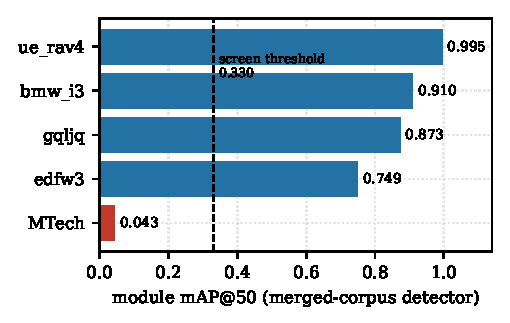
\includegraphics[width=\columnwidth]{figures/fig_screen.pdf}
\caption{Per-source module accuracy with the robust fence of Eq.~\ref{eq:screen} at
$k=3$. Two sources fall below it, one by an order of magnitude.}
\label{fig:screen}
\end{figure}

The two differ in character. The source at 0.097 lies 0.767 below the fence.
Inspection confirms the diagnosis: it annotates small internal sub-components in
extreme macro views as modules, whereas every other source annotates pack-level
modules. The detector learned the majority convention and applied it consistently, so
the collapse is a disagreement about the target, not a failure of perception. The
source at 0.641 is a milder case whose granularity index is the second highest in the
corpus but does not exceed the training-free fence, so the two screens disagree about
it and the model-based screen is the more sensitive. Three sources were excluded for
contributing fewer than 100 module instances; one of them annotates busbars
exclusively, which the screen surfaces without manual inspection.

\subsection{Agreement of the training-free screen}
\label{sec:res-screen-free}
Eq.~\ref{eq:granularity} was evaluated over all 4,760 label files, using no images and
no trained model. The divergent source attains 40.7, against 15.0 for the next highest
and a corpus median of 9.00; the fence at $k=3$ is 29.02 and exactly one source
exceeds it. It is the same source the model-based procedure flags most strongly. The
two screens are methodologically independent, one measuring detector behaviour and the
other only annotation geometry, so their agreement is a second line of evidence that
the source encodes a different convention rather than harder imagery. A corpus may
therefore be screened before a detector is trained. The index detects divergence in
annotation \emph{granularity} specifically; conventions disagreeing about class
boundaries while preserving object scale would still require the model-based screen.

\subsection{Positive control}
\label{sec:res-control}
Neither screen had been tested against a case whose answer was known in advance. A
consensus source was therefore relabelled to a deliberately different convention,
every pack-level module box being replaced by a $3\times2$ grid of inset sub-component
boxes covering the same region. No image is altered and no busbar annotation touched,
so a screen responding to the manipulation responds to annotation convention alone. A
detector was retrained on the manipulated corpus under the identical budget.

Table~\ref{tab:control} presents the outcome. The manipulated source falls from 0.941
to 0.667 and crosses the fence, while no unmanipulated source moves by more than
0.050 and four move by 0.017 or less. The flagged set gains exactly one member and
loses none. On the training-free index the same source rises from 11.1 to 185.8. Both
screens therefore recover a divergence whose ground truth is known by construction,
without false positives elsewhere.

\begin{table}[t]
\caption{Positive control. A consensus source is relabelled to a sub-component
convention and the detector retrained. Module mAP@50 above, granularity index below}
\label{tab:control}
\centering\small
\setlength{\tabcolsep}{4pt}
\begin{tabular}{lccc}
\toprule
Source & Original & Manipulated & Change \\
\midrule
\multicolumn{4}{l}{\emph{model-based screen, fence 0.864 / 0.815}} \\
battery\_comp & 1.000 & 1.000 & $0.000$ \\
edfw3 & 0.982 & 0.973 & $-0.009$ \\
bmw\_i3 & 0.967 & 0.950 & $-0.017$ \\
\textbf{manipulated} & \textbf{0.941} & \textbf{0.667} & $\mathbf{-0.274}$ \\
automated & 0.641 & 0.591 & $-0.050$ \\
divergent & 0.097 & 0.097 & $0.000$ \\
\midrule
\multicolumn{4}{l}{\emph{training-free screen, fence 29.02 / 35.24}} \\
\textbf{manipulated} & \textbf{11.1} & \textbf{185.8} & $\mathbf{+174.7}$ \\
\bottomrule
\end{tabular}
\end{table}

\subsection{Architecture comparison under a matched budget}
\label{sec:res-arch}
Both multi-source models were trained for 60 epochs and scored per source under the
identical protocol (Table~\ref{tab:arch}). The result is narrow and specific. On
conventionally annotated packs the self-supervised pretrained model is marginally
\emph{worse}, at 0.955 against 0.979. On the mild outlier it scores 0.779 against
0.641, and on the divergent source 0.337 against 0.097, a factor of 3.5.
Self-supervised pretraining therefore does not detect ordinary modules more accurately
here; it degrades considerably more gracefully when the definition of the target
moves. Both architectures produce the same partition under the screen, which indicates
the procedure to be independent of the detector it is applied to.

\begin{table}[t]
\caption{Architecture comparison under a matched 60-epoch budget, module mAP@50.
Consensus is the mean over the six sources above the fence}
\label{tab:arch}
\centering\small
\begin{tabular}{lccc}
\toprule
Model & Consensus & Mild outlier & Divergent \\
\midrule
YOLO11n & \textbf{0.979} & 0.641 & 0.097 \\
RF-DETR & 0.955 & \textbf{0.779} & \textbf{0.337} \\
\bottomrule
\end{tabular}
\end{table}

\subsection{Single-source validation inverts checkpoint selection}
\label{sec:res-inversion}
A result emerged from the matched-budget runs that was not sought and bears directly
on the paper's central claim. The validation data available for this corpus is drawn
overwhelmingly from the divergent source. During training, accuracy on that split
peaked early then fell by roughly a factor of five, while both training losses
decreased monotonically. Selecting a checkpoint on that signal is therefore selecting
for the divergent convention.

Evaluated across all sources, the selected checkpoint is \emph{worse} than the final
checkpoint by 0.235 mAP@50, a relative loss of 51\%. Across three seeds the final
checkpoint attains $0.696 \pm 0.003$ and the selected checkpoint $0.461 \pm 0.018$,
so the effect is 80 times the seed spread. On the module class, 500 bootstrap
resamples give non-overlapping 95\% intervals of $[0.659, 0.808]$ and
$[0.471, 0.626]$ (Fig.~\ref{fig:inversion}). The same inversion appears in the
pretrained model, whose validation identified epoch 3 as best and epoch 60 as
substantially worse, while across sources the epoch-60 checkpoint scores 0.955 against
0.719 on consensus sources and 0.337 against 0.079 on the divergent source. The effect
is a property of single-source validation, not of one architecture.

\begin{figure}[t]
\centering
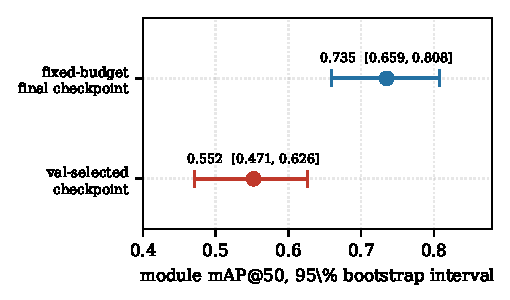
\includegraphics[width=\columnwidth]{figures/fig_inversion.pdf}
\caption{Checkpoint selection against single-source validation data. Bars are 95\%
bootstrap intervals over 500 resamples; they do not overlap.}
\label{fig:inversion}
\end{figure}

Two caveats bound the claim. The evaluation sample is drawn from the corpus rather
than held out, so later checkpoints are favoured by memorisation and the magnitude is
optimistic; what memorisation does not explain is the pattern, since memorising would
raise the final checkpoint uniformly rather than gaining on consensus sources while
losing on the divergent one. And the finding concerns validation drawn from a single
divergent source, not well-constructed validation splits.

\subsection{Deployment cost and zero-shot transfer}
Evaluated on 17 pack families absent from the corpus, drawn from an unlabelled public
collection, the merged-corpus detector attains a mean detection rate of 0.76 and finds
busbars in 16 of 17, with 1.00 on BMW i4 and Hyundai Ioniq against 0.27 on a Volvo
truck pack. Module geometry transfers to unseen passenger-vehicle packs while unusual
form factors remain the weak axis. Dynamic INT8 quantisation to ONNX reduced median
CPU latency from 56.3\,ms to 44.8\,ms and file size from 6.3\,MB to 3.4\,MB for a loss
of 0.007 mAP@50, measured over 20 images on an Apple M1 processor, giving roughly 22
frames per second without a graphics processor.

\subsection{Negative results}
\label{sec:negative}
Five failures constrain the design space, each reported because it was expected to
succeed. Open-vocabulary detection is unusable: YOLO-World \cite{yoloworld}, prompted
with \texttt{ev battery module} and \texttt{busbar}, attained 0.004 mAP@50. Naive
multi-source merging reduced module mAP@50 to 0.094 against a single-source baseline
of 0.818, so more data made the model worse; this motivated the screening procedure.
Automatic relabelling of the flagged source with Grounding DINO \cite{groundingdino}
recovered two of approximately five modules on clean frames and produced boxes
covering half the frame on greyscale macro imagery, so convention conflicts are not
cheaply repairable after collection. Copy-paste compositing
\cite{ghiasi2021copypaste} with synthetic glare degraded validation mAP@50
monotonically from 0.503 to 0.270 over six epochs. And prolonged fine-tuning degrades
the pretrained model, which peaked at epoch 3 or 4 in both runs and ended 27\% below
its peak: a model arriving already fitted gains nothing from a budget suited to one
trained from scratch.

\section{Limitations}
\label{sec:limits}

The 66\% loss of Section~\ref{sec:res-gap} is measured against an in-domain benchmark
that is itself the convention-divergent source, so it conflates generalisation loss
with training on an idiosyncratic convention and is an upper bound. No other result
depends on it.

Both screens are computed on a stratified sample of the corpus rather than held-out
data, because the validation split available here spans only two sources and cannot
support a per-source outlier test. Absolute values are optimistic and later
checkpoints are additionally favoured by memorisation; only relative orderings are
used. A held-out multi-source split would give cleaner magnitudes.

YOLO11n was trained with three seeds, giving a standard deviation of 0.003. The
pretrained model was trained once at the full budget for reasons of compute; a second
run reproduced its early-peak behaviour but was halted at epoch 9, so its numbers
carry no variance estimate.

The screening procedure requires divergent sources to be a minority, since the median
defines the consensus, and requires a minimum instance count per source; three sources
here fall below that floor and are excluded rather than reported. It would need
modification for a corpus in which two or more incompatible conventions are each well
represented.

The benchmark inherits its sources' annotation conventions and no independently
relabelled gold subset was constructed, so model error and label error cannot be
separated on it. This is material for a study whose central claim concerns annotation
quality. The corpus is assembled from public sources, so coverage is uneven and
licences vary; one source at 24\% of training images is CC BY-NC-SA 4.0 with a
propagating ShareAlike condition, and one further source became unavailable during
this study. Finally, busbar accuracy is not sufficient for autonomous operation, and
these results characterise the failure modes of the task rather than deliver a
deployable detector.

\section{Conclusion}

This paper presented a cross-facility corpus and benchmark for electric vehicle
battery component detection, and used it to establish that annotation convention,
rather than architecture, is the dominant failure mode in this application.
Per-source accuracy for one detector spans 0.097 to 1.000, and the collapse occurs
where a source disagrees about what the target class denotes rather than where the
imagery is hard. The proposed screening procedure identifies such sources from a
single training run, and a training-free variant computed from annotation geometry
identifies the same source with no training at all. Both pass a positive control in
which a relabelled consensus source is recovered while no other source changes status.

Two results about method follow. Under a matched budget, self-supervised pretraining
is marginally worse on conventionally annotated packs and better by a factor of 3.5
under annotation shift, which narrows the circumstances in which it should be
preferred to graceful degradation rather than accuracy. And validation data drawn from
a single divergent source inverts checkpoint selection, costing 51\% relative
accuracy, in both architectures tested.

Dataset design, and specifically agreement on annotation convention before collection,
is therefore the first thing to get right in this application, and the same
disagreement propagates silently into model selection if the validation split is not
itself checked. Future work will construct an independently relabelled gold subset in
order to separate model error from label error, and will repeat both screens on a
held-out multi-source split.

\section*{Acknowledgements}
The authors thank the RESCu-M2 research hub at the University of Birmingham, and
Prof. Samia Nefti-Meziani for her leadership of it, for supporting this work and
providing access to the EV battery disassembly facility.

\begin{thebibliography}{00}

\bibitem{ec_crm} European Commission, ``Study on the critical raw materials for
the EU: Final report,'' Publ. Office Eur. Union, Brussels, 2023.

\bibitem{harper2019} G. Harper \emph{et al.}, ``Recycling lithium-ion batteries
from electric vehicles,'' \emph{Nature}, vol. 575, pp. 75--86, 2019.

\bibitem{te2024} Transport \& Environment, ``From waste to value: the potential
for battery recycling in Europe,'' Brussels, 2024.

\bibitem{zang2024robotic} Y. Zang, M. Qu, D. T. Pham, R. Dixon, F. Goli,
Y. Zhang, and Y. Wang, ``Robotic disassembly of electric vehicle batteries:
Technologies and opportunities,'' \emph{Comput. Ind. Eng.}, vol. 198, 110727,
2024.

\bibitem{wegener2015} K. Wegener, S. Andrew, A. Raatz, K. Dr\"oder, and
C. Herrmann, ``Disassembly of electric vehicle batteries using the example of the
Audi Q5 hybrid system,'' \emph{Procedia CIRP}, vol. 23, pp. 155--160, 2014.

\bibitem{tan2025screws} M. Tan, J. Huang, X. Jiang, Y. Fang, Q. Liu, and
D. T. Pham, ``Robotic removal and collection of screws in collaborative
disassembly of end-of-life electric vehicle batteries,'' \emph{Biomimetics},
vol. 10, no. 8, 553, 2025.

\bibitem{screwrcnn2021} X. Li, M. Li, Y. Wu, D. Zhou, T. Liu, F. Hao, J. Yue,
and Q. Ma, ``Accurate screw detection method based on faster R-CNN and rotation
edge similarity for automatic screw disassembly,'' \emph{Int. J. Comput. Integr.
Manuf.}, vol. 34, no. 11, pp. 1177--1195, 2021.

\bibitem{screwbatt2023} H. Li, H. Zhang, Y. Zhang, S. Zhang, Y. Peng, Z. Wang,
H. Song, and M. Chen, ``An accurate activate screw detection method for automatic
electric vehicle battery disassembly,'' \emph{Batteries}, vol. 9, no. 3, 187, 2023.

\bibitem{screwcompare2026} A. Naseri, S. Khwajazada, and S. Yang, ``Comparative
analysis of YOLO and faster R-CNN models for EV battery screw detection,''
\emph{Int. J. Adv. Manuf. Technol.}, vol. 144, no. 1--2, pp. 1107--1119, 2026.

\bibitem{cvmodule2023} E. Gerlitz, L.-E. Enslin, and J. Fleischer, ``Computer
vision application for industrial Li-ion battery module disassembly,''
\emph{Prod. Eng.}, vol. 18, no. 3--4, pp. 393--401, 2023.

\bibitem{recht2019} B. Recht, R. Roelofs, L. Schmidt, and V. Shankar, ``Do
ImageNet classifiers generalize to ImageNet?,'' in \emph{Proc. ICML}, 2019,
pp. 5389--5400.

\bibitem{koh2021wilds} P. W. Koh \emph{et al.}, ``WILDS: A benchmark of
in-the-wild distribution shifts,'' in \emph{Proc. ICML}, 2021, pp. 5637--5664.

\bibitem{northcutt2021} C. G. Northcutt, A. Athalye, and J. Mueller, ``Pervasive
label errors in test sets destabilize machine learning benchmarks,'' in
\emph{Proc. NeurIPS Datasets and Benchmarks}, 2021.

\bibitem{lin2014coco} T.-Y. Lin, M. Maire, S. Belongie, J. Hays, P. Perona,
D. Ramanan, P. Doll\'ar, and C. L. Zitnick, ``Microsoft COCO: Common objects in
context,'' in \emph{Proc. ECCV}, 2014, pp. 740--755.

\bibitem{yoloworld} T. Cheng, L. Song, Y. Ge, W. Liu, X. Wang, and Y. Shan,
``YOLO-World: Real-time open-vocabulary object detection,'' in \emph{Proc. IEEE/CVF
CVPR}, 2024.

\bibitem{groundingdino} S. Liu, Z. Zeng, T. Ren \emph{et al.}, ``Grounding DINO:
Marrying DINO with grounded pre-training for open-set object detection,'' in
\emph{Proc. ECCV}, 2024.

\bibitem{ghiasi2021copypaste} G. Ghiasi, Y. Cui, A. Srinivas, R. Qian, T.-Y. Lin,
E. D. Cubuk, Q. V. Le, and B. Zoph, ``Simple copy-paste is a strong data augmentation
method for instance segmentation,'' in \emph{Proc. IEEE/CVF CVPR}, 2021,
pp. 2917--2927.

\bibitem{katiyar2026mvml} S. A. Katiyar, P. Venigalla, K. Kosimov, and
S. Nefti-Meziani, ``Vision model for detection and condition assessment of EV
battery components for circular manufacturing,'' in \emph{Proc. 12th World Congr.
Elect. Eng. Comput. Syst. Sci. (EECSS)}, London, UK, 2026, Paper MVML 125.

\bibitem{bergmann2019mvtec} P. Bergmann, M. Fauser, D. Sattlegger, and C. Steger,
``MVTec AD: A comprehensive real-world dataset for unsupervised anomaly
detection,'' in \emph{Proc. IEEE/CVF CVPR}, 2019, pp. 9592--9600.

\bibitem{carion2020detr} N. Carion, F. Massa, G. Synnaeve, N. Usunier,
A. Kirillov, and S. Zagoruyko, ``End-to-end object detection with transformers,''
in \emph{Proc. ECCV}, 2020, pp. 213--229.

\bibitem{zhou2022dg} K. Zhou, Z. Liu, Y. Qiao, T. Xiang, and C. C. Loy, ``Domain
generalization: A survey,'' \emph{IEEE Trans. Pattern Anal. Mach. Intell.},
vol. 45, no. 4, pp. 4396--4415, 2023.

\bibitem{penquitt2026} S. Penquitt, J. Klees, R. Cakaj, D. Kondermann,
M. Rottmann, and L. Schmarje, ``From label error detection to correction: A modular
framework and benchmark for object detection datasets,'' in \emph{Proc. 21st Int.
Conf. Comput. Vis. Theory Appl. (VISAPP)}, 2026.

\bibitem{abouakar2026} C. Abou Akar, H. Koubeissy, J. Khalil, J. Tekli,
M. Kamradt, and A. Makhoul, ``Rendered vs AI-generated vs real data: Training
industrial object detection models with multi-source data,'' in \emph{Proc. 21st
Int. Conf. Comput. Vis. Theory Appl. (VISAPP)}, 2026, pp. 276--287.

\bibitem{dinov2} M. Oquab \emph{et al.}, ``DINOv2: Learning robust visual
features without supervision,'' \emph{Trans. Mach. Learn. Res.}, 2024.

\bibitem{rfdetr} Roboflow, ``RF-DETR: A real-time detection transformer,'' 2025.

\bibitem{yolo11} G. Jocher and J. Qiu, ``Ultralytics YOLO11,'' 2024.

\end{thebibliography}

\end{document}
